\documentclass[
11pt, % The default document font size, options: 10pt, 11pt, 12pt
%codirector, % Uncomment to add a codirector to the title page
]{charter} 


% El títulos de la memoria, se usa en la carátula y se puede usar el cualquier lugar del documento con el comando \ttitle
\titulo{Desarrollo de un Sistema de Comunicación para Satélites basado en estándares espaciales} 

% Nombre del posgrado, se usa en la carátula y se puede usar el cualquier lugar del documento con el comando \degreename
\posgrado{Carrera de Especialización en Sistemas Embebidos} 
%\posgrado{Carrera de Especialización en Internet de las Cosas} 
%\posgrado{Carrera de Especialización en Inteligencia Artificial}
%\posgrado{Maestría en Sistemas Embebidos} 
%\posgrado{Maestría en Internet de las cosas}

% Tu nombre, se puede usar el cualquier lugar del documento con el comando \authorname
% IMPORTANTE: no omitir titulaciones ni tildación en los nombres, también se recomienda escribir los nombres completos (tal cual los tienen en su documento)
\autor{Ing. Gonzalo Lavigna}

% El nombre del director y co-director, se puede usar el cualquier lugar del documento con el comando \supname y \cosupname y \pertesupname y \pertecosupname
\director{Ing. Roberto Cibils}
\pertenenciaDirector{FIUBA} 
\codirector{} % para que aparezca en la portada se debe descomentar la opción codirector en los parámetros de documentclass
\pertenenciaCoDirector{FIUBA}

% Nombre del cliente, quien va a aprobar los resultados del proyecto, se puede usar con el comando \clientename y \empclientename
%\cliente{Gonzalo Lavigna}
%\empresaCliente{Responsable}
 
\fechaINICIO{4 de marzo de 2025}		%Fecha de inicio de la cursada de GdP \fechaInicioName
\fechaFINALPlan{22 de abril de 2025} 	%Fecha de final de cursada de GdP
\fechaFINALTrabajo{diciembre de 2025}	%Fecha de defensa pública del trabajo final


\begin{document}

\maketitle
\thispagestyle{empty}
\pagebreak


\thispagestyle{empty}
{\setlength{\parskip}{0pt}
\tableofcontents{}
}
\pagebreak


\section*{Registros de cambios}
\label{sec:registro}


\begin{table}[ht]
\label{tab:registro}
\centering
\begin{tabularx}{\linewidth}{@{}|c|X|c|@{}}
\hline
\rowcolor[HTML]{C0C0C0} 
Revisión & \multicolumn{1}{c|}{\cellcolor[HTML]{C0C0C0}Detalles de los cambios realizados} & Fecha      \\ \hline
0      & Creación del documento                                 &\fechaInicioName \\ \hline
1      & Se completa hasta el punto 5 inclusive                 & {16} de {marzo} de 2025 \\ \hline  
2      & Se completa hasta el punto 9 inclusive                 & {27} de {marzo} de 2025 \\ \hline  

%		  Se puede agregar algo más \newline
%		  En distintas líneas \newline
%		  Así                                                    & {día} de {mes} de 202X \\ \hline
%3      & Se completa hasta el punto 12 inclusive                & {día} de {mes} de 202X \\ \hline
%4      & Se completa el plan	                                 & {día} de {mes} de 202X \\ \hline

% Si hay más correcciones pasada la versión 4 también se deben especificar acá

\end{tabularx}
\end{table}

\pagebreak



\section*{Acta de constitución del proyecto}
\label{sec:acta}

\begin{flushright}
Buenos Aires, \fechaInicioName
\end{flushright}

\vspace{2cm}

Por medio de la presente, se acuerda con el \authorname\hspace{1px} que su Trabajo Final de la \degreename\hspace{1px} se titulará ``\ttitle'' y consistirá en la implementación de un prototipo de comunicación satelital basado en normas CCSDS con una FPGA. El trabajo tendrá un presupuesto preliminar estimado de 640 horas y un costo estimado de mil dólares estadounidenses (U\$D 1000), con fecha de inicio el \fechaInicioName\hspace{1px} y fecha de presentación pública en \fechaFinalName.

Se adjunta a esta acta la planificación inicial.

\vfill

% Esta parte se construye sola con la información que hayan cargado en el preámbulo del documento y no debe modificarla
\begin{table}[ht]
\centering
\begin{tabular}{ccc}
\begin{tabular}[c]{@{}c@{}}Dr. Ing. Ariel Lutenberg \\ Director posgrado FIUBA\end{tabular} & \hspace{2cm} & \begin{tabular}[c]{@{}c@{}} \supname \\ Director del Trabajo Final\end{tabular} \vspace{2.5cm} \\ 
%\multicolumn{3}{c}{\begin{tabular}[c]{@{}c@{}} \supname \\ Director del Trabajo Final\end{tabular}} \vspace{2.5cm} \\
\end{tabular}
\end{table}




\section{1. Descripción técnica-conceptual del proyecto a realizar}
\label{sec:descripcion}

El presente proyecto aborda el diseño y la implementación de un sistema digital para comunicaciones satelitales, basado en el estándar internacional establecido por el \textit{Consultative Committee for Space Data Systems} (CCSDS). La motivación principal radica en la creciente demanda de soluciones estandarizadas y confiables para la comunicación satelital, especialmente orientadas a pequeños satélites y misiones espaciales de bajo presupuesto, donde las soluciones tradicionales resultan prohibitivas en términos de costo y complejidad.

Este proyecto se enmarca en un esfuerzo personal y académico, como Trabajo Final de la Carrera de Especialización en Sistemas Embebidos. No existen condiciones especiales relacionadas con financiamiento externo, acuerdos de confidencialidad o propiedad intelectual específica y el objetivo es proporcionar un prototipo abierto y documentado para futuras implementaciones en diferentes organizaciones interesadas en el ámbito aeroespacial.

El desafío principal radica en implementar eficientemente las especificaciones del estándar CCSDS en \textit{hardware} \textit{Field-Programmable Gate Array} (FPGA), cumpliendo estrictos requerimientos de confiabilidad, robustez y eficiencia energética. El estado del arte actual muestra diversas implementaciones, generalmente complejas y costosas, orientadas a satélites de mayor tamaño o con mayores recursos disponibles. Este proyecto propone un enfoque simplificado y eficiente que destaca por su simplicidad, accesibilidad económica y facilidad de integración en satélites pequeños.

En la figura \ref{fig:diagBloques} se presenta el diagrama en bloques del sistema, compuesto por los siguientes módulos principales:
\begin{itemize}
	\item Ethernet: interfaz fisica externa \textit{ethernet} aquí es donde la FPGA se conecta con \textit{hardware} externo,ya sea una estación terrena o una red local.
	\item \textit{Universal Asynchronous Receiver-Transmitter} (UART): es la interfaz de comunicación serial que sirve típicamente para enviar comandos al FPGA y recibir datos del estado del sistema, desde una PC o terminal externa.
	\item Bloque Ethernet: gestiona la comunicación de datos \textit{ethernet} a nivel digital dentro de la FPGA. Convierte las señales físicas Ethernet en datos digitales que puedan ser procesados internamente por el sistema y viceversa.
	\item Control: se encarga del manejo interno de comandos recibidos desde el bloque UART y la generación de datos de estado del sistema. Es el bloque de gestión de mensajes, comandos y monitoreo del sistema. 
	\item Enrutador de paquetes: este bloque cumple la función de distribución y conmutación interna. Es decir, recibe paquetes de datos Ethernet desde el bloque Ethernet y determina hacia dónde dirigirlos: hacia la cadena transmisora (codificador CCSDS) o la cadena receptora (decodificador CCSDS).
	\item Transformación CCSDS: convierte los datos desde el formato Ethernet hacia tramas del estándar CCSDS \textit{Advanced Orbiting Systems} (AOS). Básicamente, consiste es una traducción hacia el protocolo estandarizado espacial.
	\item Codificador CCSDS : codifica las tramas CCSDS AOS generadas previamente, añadiendo información adicional para detección y corrección de errores (usualmente utilizando Reed-Solomon). Este bloque asegura robustez y confiabilidad en la comunicación.
	\item Modulador: acondiciona las tramas codificadas digitalmente para simular su transmisión hacia un canal físico. En este caso, realiza una modulación lógica que simula el comportamiento real de transmisión.
	\item Decodificador CCSDS: decodifica las tramas recibidas, verificando su integridad y corrigiendo errores mediante los códigos Reed-Solomon introducidos por el codificador CCSDS.
	\item Transformación Ethernet: convierte nuevamente las tramas CCSDS AOS decodificadas hacia paquetes Ethernet, facilitando así su distribución posterior hacia interfaces externas o internas.
\end{itemize}

\begin{figure}[htpb]
\centering 
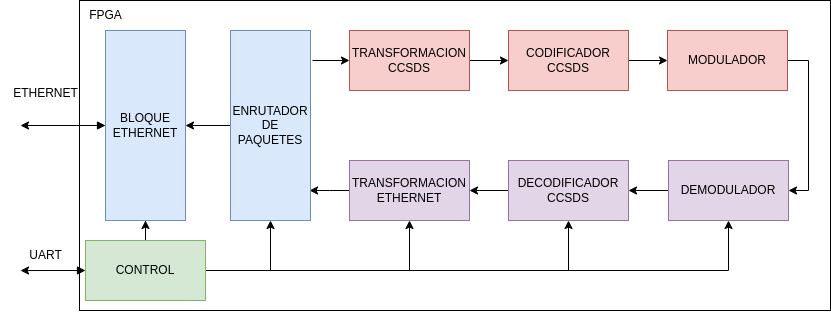
\includegraphics[width=1\textwidth]{./Figuras/TESIS_GONZALO.drawio.png}
\caption{Diagrama en bloques del sistema.}
\label{fig:diagBloques}
\end{figure}

%\vspace{25px}


Este proyecto se encuentra en una etapa inicial del ciclo de vida, enfocándose en la validación mediante simulaciones en un entorno controlado previo a cualquier implementación física más avanzada.

El cliente objetivo lo constituyen organizaciones o investigadores dedicados al desarrollo de misiones satelitales pequeñas, quienes valoran soluciones abiertas, económicas y estandarizadas para facilitar la integración y reducir riesgos en sus misiones.

La innovación principal del proyecto reside en simplificar el estándar CCSDS para aplicaciones de bajo costo y alta eficiencia, facilitando su adopción y garantizando interoperabilidad en futuras misiones espaciales.

\section{2. Identificación y análisis de los interesados}
\label{sec:interesados}

\begin{table}[ht]
%\caption{Identificación de los interesados}
%\label{tab:interesados}
\begin{tabularx}{\linewidth}{@{}|l|X|X|l|@{}}
\hline
\rowcolor[HTML]{C0C0C0} 
Rol           & Nombre y Apellido & Organización 	& Puesto 	\\ \hline
%Auspiciante   & -                 & -              	& -        	\\ \hline
Cliente       & -                 & -               & -        	\\ \hline
%Impulsor      & -                 & -              	& -       	\\ \hline
Responsable   & \authorname       & FIUBA        	& Alumno 	\\ \hline
Colaboradores & -                 & -              	& -       	\\ \hline
Orientador    & \supname	      & \pertesupname 	& Director del Trabajo Final \\ \hline
%Equipo        & -
%			  & -                 & -               	\\ \hline
%Opositores    & -                 & -              	& -        	\\ \hline
Usuario final & Industria satelital & -             	& -       	\\ \hline
\end{tabularx}
\end{table}

\vspace{25px}

\begin{itemize}
	\item Orientador: el Ing. Roberto Cibils es experto en la temática y va a ayudar con la definición de los requerimientos y el desarrollo del \textit{firmware} del embebido. Roberto Cibils cuenta con basta experiencia en sistemas robustos para aplicaciones espaciales y calificación de partes.
	\item Responsable: será quien dispondrá del conocimiento y desarrollo del proyecto.
	\item Usuario final: el usuario final de este proyecto serían principalmente, ingenieros, universidades y organizaciones dedicadas al desarrollo e implementación de misiones satelitales, especialmente aquellas orientadas a pequeños satélites o misiones de bajo costo.
\end{itemize}

\section{3. Propósito del proyecto}
\label{sec:proposito}

El propósito del proyecto es el desarrollo de un prototipo de un sistema de comunicación basado en el estándar CCSDS dentro de una FPGA. Tiene como objetivo proporcionar una solución tecnológica eficiente y accesible para aplicaciones satelitales, especialmente orientada a misiones de satélites pequeños y de bajo costo. De esta forma, se pretende reducir significativamente la complejidad y los costos asociados a sistemas tradicionales, favoreciendo la investigación, el desarrollo y el despliegue de futuras misiones espaciales por parte de organizaciones académicas y científicas.

\section{4. Alcance del proyecto}
\label{sec:alcance}

El presente proyecto incluye:
\begin{itemize}
	\item Diseño e implementación de un sistema digital de comunicación satelital basado en el estándar CCSDS.
	\item Integración de algoritmos de codificación y decodificación Reed-Solomon según CCSDS.
	\item Desarrollo integral del sistema sobre una placa de desarrollo de FPGA.
	\item Simulación del canal de comunicación utilizando un esquema de \textit{loopback} lógico.
	\item Validación funcional mediante herramientas de simulación.
	\item Validación de la implementación utilizando herramientas de síntesis como Vivado.
	\item Desarrollo de una interfaz mínima utilizando UART para control y monitoreo del sistema.
	\item Documentación técnica completa del diseño y código fuente.
	\item Liberación del código bajo licencia de código abierto.
\end{itemize}

El presente proyecto no incluye:
\begin{itemize}
	\item Implementación física de \textit{hardware} de radiofrecuencia (RF), ni diseño de antenas.
	\item Integración real con \textit{hardware} satelital.
	\item Realización de pruebas en ambientes espaciales reales o estaciones terrenas operativas.
	\item Desarrollo de software adicional para análisis avanzado o procesamiento de datos fuera del alcance del sistema propuesto.
	\item Utilización de conversor analógico digital.
	\item Utilización de conversor digital analógico.
\end{itemize}

\section{5. Supuestos del proyecto}
\label{sec:supuestos}

Para el desarrollo del presente proyecto se supone que:

\begin{itemize}
	\item Disponibilidad de recursos:
	\begin{itemize}	
		\item Se dispondrá oportunamente de una placa de desarrollo que contenga una FPGA.
		\item Cable \textit{Universal Serial Bus} USB a UART, que permitirá establecer comunicación entre la FPGA y una terminal externa (por ejemplo, una computadora).
		\item Cable Ethernet (categoría 5e o superior), con conectores RJ-45 en ambos extremos.
		\item El proyecto contempla la utilización de módulos proporcionados por terceros para realizar las funciones específicas de codificación y decodificación Reed-Solomon según lo establecido en el estándar CCSDS. Estos módulos externos, previamente validados y disponibles abiertamente, permitirán acelerar el desarrollo del sistema.
	\end{itemize}
	
	\item Experiencia técnica:
	\begin{itemize}	
		\item El responsable posee un nivel adecuado de conocimiento y experiencia previa en leguajes de descripción de \textit{hardware} como VHDL o Verilog, necesarios para el diseño, implementación y validación lógica del sistema propuesto.
		\item El responsable dispone de la capacidad técnica para integrar y validar adecuadamente módulos de terceros, como los bloques de codificación y decodificación Reed-Solomon.
		\item El responsable cuenta con conocimientos sólidos en el manejo del estándar CCSDS y familiaridad con las herramientas de desarrollo FPGA, como Vivado y ModelSim.
		\item Se dispondrán de las 640 horas requeridas para realizar el proyecto.
		
	\end{itemize}
	
	
\end{itemize}

\section{6. Requerimientos}
\label{sec:requerimientos}



\begin {enumerate}
	\item Requerimientos funcionales:
		\begin{enumerate}
			\item El sistema debe tener una baja latencia en el procesamiento y transferencia de paquetes (menor a 15 ms).				
			\item El usuario debe ser capaz de configurar todos los bloques del sistema a través de comando externos utilizando UART.
			\item El bloque Ethernet debe soportar transmisión y recepción de paquetes estándar de Ethernet (IEEE 802.3).
			\item El bloque Ethernet debe soportar una velocidad de comunicación de 100 Mbps.
			\item El bloque Ethernet debe tener la capacidad de manejar en simultáneo múltiples paquetes entrantes y salientes.
			\item El bloque Ethernet debe tener la capacidad de generar estadísticas básicas de red: paquetes transmitidos, paquetes recibidos, errores detectados.					
			\item El bloque Ethernet debe tener la capacidad de identificar y gestionar errores básicos en paquetes Ethernet.
			\item El bloque Ethernet debe brindar soporte para tramas Ethernet estándar de hasta 1500 bytes (\textit{Maximum Transmission Unit} estándar).
			\item El bloque enrutador debe ser capaz de recibir, procesar y enrutar paquetes Ethernet internamente entre los diferente módulos del sistema.
			\item El bloque enrutador debe tener la capacidad de almacenamiento temporal de unos 4 paquetes para evitar la pérdida de datos en situaciones de congestión temporal.
			\item El bloque enrutador deberá contar con un mecanismo interno para realizar una conexión logica en modo \textit{loopback}, permitiendo que los paquetes Ethernet recibidos puedan ser automáticamente redirigidos a la cadena de transmisión de datos Ethernet. Este mecanismo facilitará pruebas y validaciones funcionales.
			\item El sistema debe encapsular correctamente los paquetes Ethernet recibidos en tramas AOS según especificaciones del estándar CCSDS 732.0-B.
			\item El sistema debe ser capaz de codificar y decodificar tramas CCSDS completas agregando códigos Reed-Solomon para detección y corrección de errores, según la configuración estándar (255,239).
			\item El bloque modulador debe implementar un esquema de modulación digital compatible con los estándares utilizados en sistemas espaciales CCSDS: \textit{Binary Phase Shift Keying} (BPSK) y \textit{Quadrature Phase Shift Keying} (QPSK) según lo especificado en el estándar CCSDS 401.0-B.			
		\end{enumerate}	
	\item Requerimientos de documentación:
		\begin{enumerate}
			\item Toda la documentación técnica del proyecto, incluyendo diagramas, especificaciones, manuales de usuario, y procedimientos de validación y configuración, deberán estar claramente redactados en español, utilizando un lenguaje formal y técnico.
			\item La totalidad del código fuente generado, junto con su documentación asociada, deberá publicarse en repositorios públicos de acceso general garantizando así su disponibilidad abierta para cualquier usuario interesado.		
			\item Deberá incluirse una guía breve («README») en los repositorios públicos, que describa claramente el objetivo, características principales y licencia de uso.
			\item Todo el código fuente generado en este proyecto, junto con su documentación asociada, deberá publicarse bajo la licencia de código abierto BSD de 3 cláusulas. Esta licencia permite explícitamente el uso libre, modificación, distribución y comercialización del software y derivados.
		\end{enumerate}				
	\item Requerimientos de verificación y validación:
		\begin{enumerate}
			\item Se deberán desarrollar bancos de pruebas específicos para cada módulo interno del sistema, utilizando lenguajes estándares como Python, VHDL o SystemVerilog, que permitan simular y verificar su correcto funcionamiento individual.
			\item Los bloques Transformación CCSDS y Transformación Ethernet se verificarán en conjunto conectando los mismos en \textit{loopback} en un banco de pruebas realizado para dicho propósito.
			\item Los bloques Codificador CCSDS y Decodificador CCSDS se verificarán en conjunto conectando los mismos en \textit{loopback} en un banco de pruebas realizado para dicho propósito.			
			\item Los bloques Modulador y Demodulador se verificarán en conjunto conectando los mismos en \textit{loopback} en un banco de pruebas realizado para dicho propósito.		
			\item Todos las simulaciones funcionales deben realizar con herramientas reconocidas como Vivado Simulator, ModelSim o herramientas equivalentes.		
			\item La verificación del sistema deberá incluir simulaciones de integración, donde se validará la interoperabilidad de los módulos interconectados mediante interfaces AXI-Stream y AXI-Lite.		
			\item La validación del sistema deberá realizarse haciendo pruebas funcionales en la placa de desarrollo en modo \textit{loopback} lógico, verificando el cumplimiento de los requisitos del estándar CCSDS y la correcta operación del flujo completo desde generación hasta recepción de datos.			
			\item Se debe incluir una simulación con la inserción controlada de errores (por ejemplo, ruido o corrupción artificial de paquetes) para verificar la robustez y la capacidad de corrección de errores del sistema implementado.						
		\end{enumerate}
				
	\item Requerimientos de interfaz:
		\begin{enumerate}
			\item El sistema deberá contar con una interfaz UART para comunicación serie externa, que permita monitorear el estado operativo y enviar comandos básicos para configurar y controlar la operación del sistema.
			\item La interfaz UART deberá funcionar bajo una configuración estándar de comunicación (8 bits de datos, sin paridad y 1 bit de parada), soportando tasas configurables entre 9600 y 115200 baudios.
			\item Deberá incluirse una interfaz Ethernet física compatible con el estándar IEEE 802.3, para la transmisión y recepción externa de paquetes Ethernet estándar (mínimo 100 Mbps).
			\item Todos los módulos internos del sistema deberán utilizar el protocolo \textit{AXI-Stream} como estándar para la comunicación e intercambios de paquetes, asegurando así la compatibilidad, simplicidad en la integración y estandarización del flujo interno del sistema.
			\item Todos los módulos internos del sistema deberán contar con una interfaz de control y monitoreo basada en el protocolo \textit{AXI-Lite}. Esta interfaz permitirá realizar operaciones básicas de lectura y escritura en registros internos para configurar parámetros específicos de cada módulo y obtener información sobre el estado operativo en tiempo real.
		\end{enumerate}
\end{enumerate}

\section{7. Historias de usuarios (\textit{Product backlog})}
\label{sec:backlog}

Se utilizó la asignación de \textit{story points} para evaluar las historias de usuario. El valor se determinó considerando los siguientes factores: tiempo, complejidad e incertidumbre asociada con la tarea. 

\begin{itemize}
	\item Tiempo.
	\item Complejidad.
	\item Riesgo.
\end{itemize}

Para las estimaciones mediante  \textit{story points} se utilizará como escala números de la serie de Fibonacci comprendidos en el rango [1, 8]. A cada criterio se le asigna un número dentro de esta escala. Luego, se sumarán los números de cada criterio para obtener una calificación final. Si este número no pertenece a un valor de la serie se aproxima al más cercano. Un número más grande indica mayor complejidad, riesgo y/o tiempo.

\begin{itemize}
\item Historia 1: Como operador del sistema quiero monitorear el estado operativo para verificar rápidamente que el sistema funciona correctamente. Tiempo: 2 - Complejidad: 2 - Riesgo: 1 - \textit{story points}: 5.
\item Historia 2: Como ingeniero de integración, quiero una interfaz Ethernet estándar (IEEE 802.3) para enviar y recibir paquetes desde sistemas externos en pruebas y validaciones. Tiempo: 3 - Complejidad: 3 - Riesgo: 2 - \textit{story points}: 8.
\item Historia 3: Como desarrollador de FPGA, quiero que todos los módulos internos se comuniquen mediante AXI-Stream para asegurar la interoperabilidad y escalabilidad del diseño. Tiempo: 2 - Complejidad: 2 - Riesgo: 1 - \textit{story points}: 5.
\item Historia 4: Como desarrollador FPGA, quiero utilizar bloques validados de codificación y decodificación Reed-Solomon provistos por terceros para acelerar el desarrollo y reducir riesgos técnicos. Tiempo: 2 - Complejidad: 1 - Riesgo: 8 - \textit{story points}: 13.
\item Historia 5: Como ingeniero de integración, quiero realizar simulaciones en modo \textit{loopback} lógico para validar el funcionamiento completo del protocolo CCSDS sin \textit{hardware} externo adicional. Tiempo: 2 - Complejidad: 1 - Riesgo: 8 - \textit{story points}: 13.
\item Historia 6: Como usuario final , quiero acceder al código fuente y documentación completa del sistema en repositorios públicos para adaptarlo y reutilizarlo en futuras misiones satelitales. Tiempo: 1 - Complejidad: 1 - Riesgo: 1 - \textit{story points}: 3.
\item Historia 7: Como desarrollador de FPGA, quiero configurar fácilmente los módulos internos mediante AXI-Lite para adaptar rápidamente los parámetros operativos del sistema en diferentes escenarios de prueba. Tiempo: 1 - Complejidad: 3 - Riesgo: 1 - \textit{story points}: 5.
\item Historia 8: Como desarrollador de FPGA, quiero contar con bancos de prueba automatizados para realizar simulaciones rápidas y repetibles de los módulos individuales del sistema.Tiempo: 5 - Complejidad: 3 - Riesgo: 5 - \textit{story points}: 13.
\end{itemize}


\section{8. Entregables principales del proyecto}
\label{sec:entregables}

Los entregables del proyecto son:

\begin{itemize}
	\item Informe de avance del proyecto.
	\item Código fuente completo del sistema implementado (con licencia BSD-3).
	\item Bancos de pruebas utilizados para simulación y validación.
	\item Documentación técnica del diseño, diagramas y especificaciones técnicas.
	\item Manual de uso y guía rápida para configuración y operación del prototipo desarrollado.
	\item Resultados y documentación de las pruebas realizadas en placa, con el prototipo del sistema implementado y funcionando en una placa de desarrollo de FPGA.
	\item Informe final, incluyendo resultados obtenidos, análisis del desempeño, conclusiones y recomendaciones.
\end{itemize}

\section{9. Desglose del trabajo en tareas}
\label{sec:wbs}

\begin{enumerate}
\item Gestión y documentación del proyecto (100 h)
	\begin{enumerate}
	\item Definición inicial del alcance del proyecto (8 h).
	\item Revisión y aprobación del alcance definitivo (8 h).
	\item Informes preliminares de avance del proyecto (8 h).
	\item Elaboración de documentación técnica general, diagrama en bloque y documentación de la arquitectura (10 h).
	\item Escribir memoria técnica (40 h).
	\item Escribir y preparar presentación final (10 h).
	\item Crear documento de lecciones aprendidas (8 h).	
	\item Publicación de documentación en repositorios públicos (8 h).	
	\end{enumerate}
\item Diseño conceptual y arquitectura (60 h)
	\begin{enumerate}
	\item Investigación inicial de los diversos estándares CCSDS (20 h).
	\item Análisis de requerimientos técnicos CCSDS a implementar en la FPGA (20 h).
	\item Diseño conceptual del sistema (4 h).
	\item Diseño detallado del sistema y diagramas finales (16 h).
	\end{enumerate}
\item  Configuración del entorno de desarrollo (40 h)
	\begin{enumerate}
	\item Instalación y configuración inicial del software Vivado (4 h).
	\item Instalación y configuración del simulador \textit{ModelSim} o equivalente.(4 h).
	\item Preparación de proyecto inicial (estructura del proyecto, repositorios Git) (4 h).
	\item Configuración del entorno para integración continua y gestión de código fuente (28 h).
	\end{enumerate}
\item  Desarrollo de las interfaces del sistema (60 h)
	\begin{enumerate}
	\item Diseño del módulo interfaz UART (10 h).
	\item Implementación y validación módulo UART (10 h).
	\item Diseño del módulo interfaz Ethernet (20 h).
	\item Implementación y validación módulo Ethernet (20 h).		
	\end{enumerate}
\item  Implementación del protocolo AXI interno (40 h)
	\begin{enumerate}
	\item Diseño e implementación interfaces AXI-Stream (20 h).
	\item Diseño e implementación interfaces AXI-Lite (20 h).
	\end{enumerate}	
\item  Integración bloques Reed-Solomon (120 h)	
	\begin{enumerate}
	\item Integración bloque codificador Reed-Solomon (20 h).
	\item Validación y ajustes codificador Reed-Solomon (20 h).
	\item Validación cruzada del módulo codificador Reed-Solomon contra modelo Python (20 h).	
	\item Integración bloque decodificador Reed-Solomon (20 h).
	\item Validación y ajustes decodificador Reed-Solomon (20 h).
	\item Validación cruzada del módulo decodificador Reed-Solomon contra modelo Python (20 h).		
	\end{enumerate}	
	\item Implementación módulos conversión Ethernet/AOS (60 h)
	\begin{enumerate}
		\item Diseño e implementación módulo Ethernet a AOS (20 h).
		\item Pruebas módulo Ethernet a AOS (10 h).
		\item Diseño módulo AOS a Ethernet (20 h).
		\item Pruebas módulo AOS a Ethernet (10 h).
	\end{enumerate}	
	\item Implementación bloques modulación/demodulación (60 h)
	\begin{enumerate}
		\item Diseño e implementación del módulo modulador CCSDS (10 h).
		\item Pruebas módulo modulador CCSDS (10 h).
		\item Diseño e implementación del módulo demodulador CCSDS (20 h).
		\item Pruebas módulo demodulador CCSDS (20 h).
	\end{enumerate}	
	\item Validación y pruebas (100 h)
	\begin{enumerate}
		\item Diseño y desarrollo de bancos de prueba en \textit{loopback} (20 h).
		\item Ejecución y validación de bancos de prueba en \textit{loopback} (20 h).
		\item Síntesis e implementación del sistema completo en placa FPGA (40 h).
		\item Ejecución de pruebas de validación sobre el prototipo implementado (20 h).
	\end{enumerate}	
	\end{enumerate}		

Cantidad total de horas: 640.

\section{10. Diagrama de Activity On Node}
\label{sec:AoN}

\begin{consigna}{red}
Armar el AoN a partir del WBS definido en la etapa anterior.

Una herramienta simple para desarrollar los diagramas es el Draw.io (\url{https://app.diagrams.net/}).
\href{https://app.diagrams.net}{Draw.io}


\begin{figure}[htpb]
\centering 
\includegraphics[width=.8\textwidth]{./Figuras/AoN.png}
\caption{Diagrama de \textit{Activity on Node}.}
\label{fig:AoN}
\end{figure}

Indicar claramente en qué unidades están expresados los tiempos.
De ser necesario indicar los caminos semi críticos y analizar sus tiempos mediante un cuadro.
Es recomendable usar colores y un cuadro indicativo describiendo qué representa cada color.

\end{consigna}

\section{11. Diagrama de Gantt}
\label{sec:gantt}

\begin{consigna}{red}
Existen muchos programas y recursos \textit{online} para hacer diagramas de Gantt, entre los cuales destacamos:

\begin{itemize}
\item Planner
\item GanttProject
\item Trello + \textit{plugins}. En el siguiente link hay un tutorial oficial: \\ \url{https://blog.trello.com/es/diagrama-de-gantt-de-un-proyecto}
\item Creately, herramienta online colaborativa. \\\url{https://creately.com/diagram/example/ieb3p3ml/LaTeX}
\item Se puede hacer en latex con el paquete \textit{pgfgantt}\\ \url{http://ctan.dcc.uchile.cl/graphics/pgf/contrib/pgfgantt/pgfgantt.pdf}
\end{itemize}

Pegar acá una captura de pantalla del diagrama de Gantt, cuidando que la letra sea suficientemente grande como para ser legible. 
Si el diagrama queda demasiado ancho, se puede pegar primero la ``tabla'' del Gantt y luego pegar la parte del diagrama de barras del diagrama de Gantt.

Configurar el software para que en la parte de la tabla muestre los códigos del EDT (WBS).\\
Configurar el software para que al lado de cada barra muestre el nombre de cada tarea.\\
Revisar que la fecha de finalización coincida con lo indicado en el Acta Constitutiva.

En la figura \ref{fig:gantt}, se muestra un ejemplo de diagrama de gantt realizado con el paquete de \textit{pgfgantt}. 
En la plantilla pueden ver el código que lo genera y usarlo de base para construir el propio.

Las fechas pueden ser calculadas utilizando alguna de las herramientas antes citadas. Sin embargo, el siguiente ejemplo
fue elaborado utilizando 
\href{https://docs.google.com/spreadsheets/d/1fBz8NhSpc4tkkhz3KjJCbh1nR_ltDkfEcZi4tZXduqs}{esta hoja de cálculo}.

Es importante destacar que el ancho del diagrama estará dado por la longitud del texto utilizado para las tareas 
(Ejemplo: tarea 1, tarea 2, etcétera) y el valor \textit{x unit}. Para mejorar la apariencia del diagrama, es necesario
ajustar este valor y, quizás, acortar los nombres de las tareas.

\begin{figure}[htpb]
  \begin{center}
    \begin{ganttchart}[
      time slot unit=day,
      time slot format=isodate,
      x unit=0.038cm,
      y unit title=0.7cm,
      y unit chart=0.6cm,
      milestone/.append style={xscale=4}
      ]{2021-03-05}{2021-12-16}
      \gantttitlecalendar*{2021-03-05}{2021-12-16}{year} \\
      \gantttitlecalendar*{2021-03-05}{2021-12-16}{month} \\
      \ganttgroup{Duración Total}{2021-03-05}{2021-12-16} \\
      %%%%%%%%%%%%%%%%%Organización
      \ganttgroup{Organización}{2021-03-05}{2021-04-16} \\
      \ganttbar{Planificación del proyecto}{2021-03-05}{2021-04-15} \\
      %%%%%%%%%%%%%%%%%Ejecución
      \ganttgroup{Ejecución}{2021-04-16}{2021-10-21} \\
      \ganttbar{Tarea 1}{2021-04-16}{2021-04-29} \\
      \ganttbar{Tarea 2}{2021-04-30}{2021-05-13} \\
      \ganttbar{Tarea 3}{2021-05-14}{2021-05-27} \\
      \ganttbar{Tarea 4}{2021-05-28}{2021-07-12} \\
      \ganttbar{Tarea 5}{2021-07-13}{2021-08-09} \\
      \ganttbar{Tarea 6}{2021-08-10}{2021-09-23} \\
      \ganttbar{Tarea 7}{2021-09-24}{2021-09-30} \\
      \ganttbar{Tarea 8}{2021-10-01}{2021-10-14} \\
      \ganttbar{Tarea 9}{2021-10-15}{2021-10-21} \\
      % %%%%%%%%%%%%%%%%%Finalización
      \ganttgroup{Finalización}{2021-10-22}{2021-12-16} \\
      \ganttbar{Memoria v1}{2021-10-22}{2021-11-04} \\
      \ganttbar{Memoria v2}{2021-11-05}{2021-11-18} \\
      \ganttbar{Memoria final}{2021-11-19}{2021-12-02} \\
      % La fecha del siguiente milestone es la fecha en que terminamos la memoria
      \ganttmilestone{Enviar memoria al director}{2021-12-02} \\
      \ganttbar{Elaborar la presentación}{2021-12-03}{2021-12-16} \\
      \ganttmilestone{Ensayo de la presentación}{2021-12-16} \\
      %%%%%%%%%%%%%%%%%%%%%%%%%%%%%%%%%%%%%%%%%%%%%%%%%%%%%%%%%%%%%%%
    \end{ganttchart}
  \end{center}
  \caption{Diagrama de gantt de ejemplo}
  \label{fig:gantt}
\end{figure}


\begin{landscape}
\begin{figure}[htpb]
\centering 
\includegraphics[height=.85\textheight]{./Figuras/Gantt-2.png}
\caption{Ejemplo de diagrama de Gantt (apaisado).} %Modificar este título acorde.
\label{fig:diagGantt}
\end{figure}

\end{landscape}

\end{consigna}


\section{12. Presupuesto detallado del proyecto}
\label{sec:presupuesto}

\begin{consigna}{red}
Si el proyecto es complejo entonces separarlo en partes:
\begin{itemize}
	\item Un total global, indicando el subtotal acumulado por cada una de las áreas.
	\item El desglose detallado del subtotal de cada una de las áreas.
\end{itemize}

IMPORTANTE: No olvidarse de considerar los COSTOS INDIRECTOS.

Incluir la aclaración de si se emplea como moneda el peso argentino (ARS) o si se usa moneda extranjera (USD, EUR, etc). Si es en moneda extranjera se debe indicar la tasa de conversión respecto a la moneda local en una fecha dada.

\end{consigna}

\begin{table}[htpb]
\centering
\begin{tabularx}{\linewidth}{@{}|X|c|r|r|@{}}
\hline
\rowcolor[HTML]{C0C0C0} 
\multicolumn{4}{|c|}{\cellcolor[HTML]{C0C0C0}COSTOS DIRECTOS} \\ \hline
\rowcolor[HTML]{C0C0C0} 
Descripción &
  \multicolumn{1}{c|}{\cellcolor[HTML]{C0C0C0}Cantidad} &
  \multicolumn{1}{c|}{\cellcolor[HTML]{C0C0C0}Valor unitario} &
  \multicolumn{1}{c|}{\cellcolor[HTML]{C0C0C0}Valor total} \\ \hline
 &
  \multicolumn{1}{c|}{} &
  \multicolumn{1}{c|}{} &
  \multicolumn{1}{c|}{} \\ \hline
 &
  \multicolumn{1}{c|}{} &
  \multicolumn{1}{c|}{} &
  \multicolumn{1}{c|}{} \\ \hline
\multicolumn{1}{|l|}{} &
   &
   &
   \\ \hline
\multicolumn{1}{|l|}{} &
   &
   &
   \\ \hline
\multicolumn{3}{|c|}{SUBTOTAL} &
  \multicolumn{1}{c|}{} \\ \hline
\rowcolor[HTML]{C0C0C0} 
\multicolumn{4}{|c|}{\cellcolor[HTML]{C0C0C0}COSTOS INDIRECTOS} \\ \hline
\rowcolor[HTML]{C0C0C0} 
Descripción &
  \multicolumn{1}{c|}{\cellcolor[HTML]{C0C0C0}Cantidad} &
  \multicolumn{1}{c|}{\cellcolor[HTML]{C0C0C0}Valor unitario} &
  \multicolumn{1}{c|}{\cellcolor[HTML]{C0C0C0}Valor total} \\ \hline
\multicolumn{1}{|l|}{} &
   &
   &
   \\ \hline
\multicolumn{1}{|l|}{} &
   &
   &
   \\ \hline
\multicolumn{1}{|l|}{} &
   &
   &
   \\ \hline
\multicolumn{3}{|c|}{SUBTOTAL} &
  \multicolumn{1}{c|}{} \\ \hline
\rowcolor[HTML]{C0C0C0}
\multicolumn{3}{|c|}{TOTAL} &
   \\ \hline
\end{tabularx}%
\end{table}


\section{13. Gestión de riesgos}
\label{sec:riesgos}

\begin{consigna}{red}
a) Identificación de los riesgos (al menos cinco) y estimación de sus consecuencias:
 
Riesgo 1: detallar el riesgo (riesgo es algo que si ocurre altera los planes previstos de forma negativa)
\begin{itemize}
	\item Severidad (S): mientras más severo, más alto es el número (usar números del 1 al 10).\\
	Justificar el motivo por el cual se asigna determinado número de severidad (S).
	\item Probabilidad de ocurrencia (O): mientras más probable, más alto es el número (usar del 1 al 10).\\
	Justificar el motivo por el cual se asigna determinado número de (O). 
\end{itemize}   

Riesgo 2:
\begin{itemize}
	\item Severidad (S): X.\\
	Justificación...
	\item Ocurrencia (O): Y.\\
	Justificación...
\end{itemize}

Riesgo 3:
\begin{itemize}
	\item Severidad (S):  X.\\
	Justificación...
	\item Ocurrencia (O): Y.\\
	Justificación...
\end{itemize}


b) Tabla de gestión de riesgos:      (El RPN se calcula como RPN=SxO)

\begin{table}[htpb]
\centering
\begin{tabularx}{\linewidth}{@{}|X|c|c|c|c|c|c|@{}}
\hline
\rowcolor[HTML]{C0C0C0} 
Riesgo & S & O & RPN & S* & O* & RPN* \\ \hline
       &   &   &     &    &    &      \\ \hline
       &   &   &     &    &    &      \\ \hline
       &   &   &     &    &    &      \\ \hline
       &   &   &     &    &    &      \\ \hline
       &   &   &     &    &    &      \\ \hline
\end{tabularx}%
\end{table}

Criterio adoptado: 

Se tomarán medidas de mitigación en los riesgos cuyos números de RPN sean mayores a...

Nota: los valores marcados con (*) en la tabla corresponden luego de haber aplicado la mitigación.

c) Plan de mitigación de los riesgos que originalmente excedían el RPN máximo establecido:
 
Riesgo 1: plan de mitigación (si por el RPN fuera necesario elaborar un plan de mitigación).
  Nueva asignación de S y O, con su respectiva justificación:
  \begin{itemize}
	\item Severidad (S*): mientras más severo, más alto es el número (usar números del 1 al 10).
          Justificar el motivo por el cual se asigna determinado número de severidad (S).
	\item Probabilidad de ocurrencia (O*): mientras más probable, más alto es el número (usar del 1 al 10).
          Justificar el motivo por el cual se asigna determinado número de (O).
	\end{itemize}

Riesgo 2: plan de mitigación (si por el RPN fuera necesario elaborar un plan de mitigación).
 
Riesgo 3: plan de mitigación (si por el RPN fuera necesario elaborar un plan de mitigación).

\end{consigna}


\section{14. Gestión de la calidad}
\label{sec:calidad}

\begin{consigna}{red}
Elija al menos diez requerimientos que a su criterio sean los más importantes/críticos/que aportan más valor y para cada uno de ellos indique las acciones de verificación y validación que permitan asegurar su cumplimiento.

\begin{itemize} 
\item Req \#1: copiar acá el requerimiento con su correspondiente número.

\begin{itemize}
	\item Verificación para confirmar si se cumplió con lo requerido antes de mostrar el sistema al cliente. Detallar.
	\item Validación con el cliente para confirmar que está de acuerdo en que se cumplió con lo requerido. Detallar. 
\end{itemize}

\end{itemize}

Tener en cuenta que en este contexto se pueden mencionar simulaciones, cálculos, revisión de hojas de datos, consulta con expertos, mediciones, etc.  

Las acciones de verificación suelen considerar al entregable como ``caja blanca'', es decir se conoce en profundidad su funcionamiento interno.  

En cambio, las acciones de validación suelen considerar al entregable como ``caja negra'', es decir, que no se conocen los detalles de su funcionamiento interno.

\end{consigna}

\section{15. Procesos de cierre}    
\label{sec:cierre}

\begin{consigna}{red}
Establecer las pautas de trabajo para realizar una reunión final de evaluación del proyecto, tal que contemple las siguientes actividades:

\begin{itemize}
	\item Pautas de trabajo que se seguirán para analizar si se respetó el Plan de Proyecto original:\\
	 - Indicar quién se ocupará de hacer esto y cuál será el procedimiento a aplicar. 
	\item Identificación de las técnicas y procedimientos útiles e inútiles que se emplearon, los problemas que surgieron y cómo se solucionaron:\\
	 - Indicar quién se ocupará de hacer esto y cuál será el procedimiento para dejar registro.
	\item Indicar quién organizará el acto de agradecimiento a todos los interesados, y en especial al equipo de trabajo y colaboradores:\\
	  - Indicar esto y quién financiará los gastos correspondientes.
\end{itemize}

\end{consigna}

\end{document}
